\section{Device Discovery}
This section discusses important aspects or problems of the device discovery process.
This refers to both the ESP-NOW discovery process and the network discovery process.


    \subsection{Network Discovery} \label{sec:network_discovery}
    For discovering the Raspberry Pi on the ESP and vice versa,
    IP's need to be exchanged. This was tried in two ways:
        \subsubsection{By Hostname}
        The first approach was to set a hostname for the 
        ESP32 and fetch data through it. While this worked
        in most networks, it isn't possible or needs to 
        configured in some, which would make the average 
        consumer unable to make use of the system.

        \subsubsection{Via UDP Broadcast}
        The second approach was to broadcast the IP of the ESP32
        via UDP-Broadcast. This would send a 
        message into the network that the Raspberry Pi
        would catch and save, this could then be used to send a
        direct HTTP-Post to the bridge to share the servers IP. 
        While sending a broadcast is
        a lot of network traffic, it is the most reliable way
        to discover the Raspberry Pi in any network. To minimize
        unintended traffic, the broadcast are only sent for a set
        period of time after boot.
        \begin{figure}
            \centering
            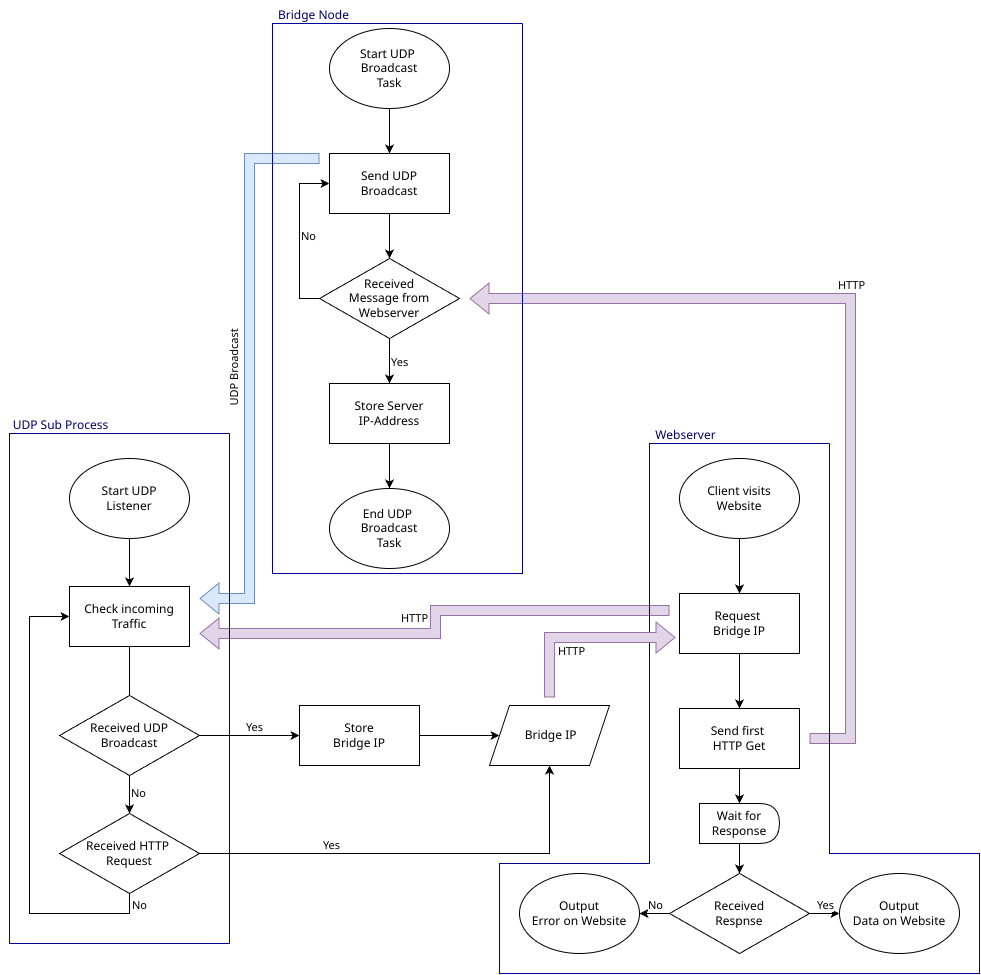
\includegraphics[width=\textwidth]{topics/flowcharts/UDP-Discovery.drawio.png}
            \caption{UDP Discovery Process}
            \label{fig:udp_discovery}
        \end{figure}

        \subsection{ESP-NOW Discovery} \label{sec:espnow_discovery}
        The ESP-NOW discovery process is a crucial part of the system. It allows the
        bridge node to discover new nodes and allows the slave nodes to find the bridge
        node. The process is as seen in the following flowchart:
        \begin{figure}
            \centering
            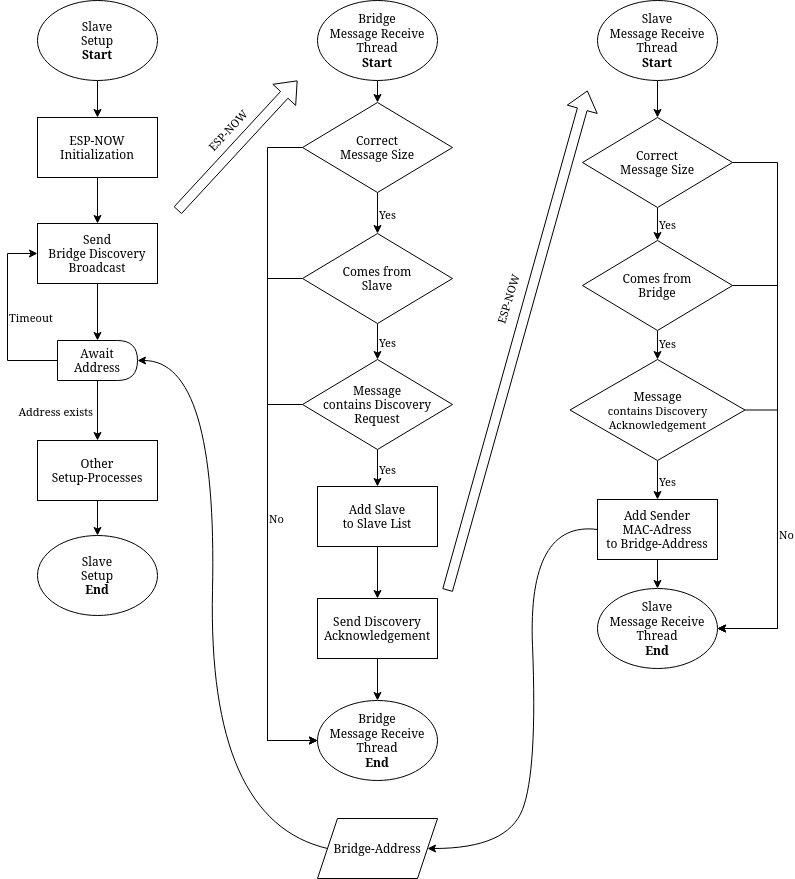
\includegraphics[width=\textwidth]{topics/flowcharts/ESP-NOW-Discovery.drawio.png}
            \caption{ESP-NOW Discovery Process}
            \label{fig:espnow_discovery}
        \end{figure}